%! Author = Thomas_normal
%! Date = 10.05.2023

% Preamble
\documentclass[11pt]{article}

% Packages

\usepackage{amsmath}
\usepackage{tikz}
\usepackage{pgfplots}

\newcommand{\TemperatureHumidityCovariance}{102.3\ ^{\circ} C g / m^3}
\newcommand{\TemperatureHumidityCorrelation}{0.8571}
\newcommand{\RegressionOffset}{(1.8 \pm 1.2)\  g / m^3}
\newcommand{\RegressionSlope}{(0.343 \pm 0.057)\ g / m^3 / ^{\circ} C}


% Document
\begin{document}

    \title{Fr2 - Sheet 3 - Correlation}
    \author{Thomas Karb}


    \maketitle

    \section{}
    In this part we analyse the linear correlation of following weather data:
    
    \begin{table}[h!]
\centering
\begin{tabular}
{| c | c |}
\hline
 Temperature in $°C$ & Humidity in $g/m^3$ \\ 
\hline
 -15 & 0.58 \\ 
\hline
 -11 & 0.65 \\ 
\hline
 -7 & 0.96 \\ 
\hline
 -3 & 1.62 \\ 
\hline
 1 & 1.39 \\ 
\hline
 5 & 1.54 \\ 
\hline
 9 & 3.7 \\ 
\hline
 13 & 3.66 \\ 
\hline
 17 & 3.85 \\ 
\hline
 21 & 4.77 \\ 
\hline
 25 & 6.16 \\ 
\hline
 29 & 9.43 \\ 
\hline
 33 & 13.48 \\ 
\hline
 37 & 16.4 \\ 
\hline
 41 & 25.49 \\ 
\hline
\end{tabular}
\label{tab:EnvironmentData}
\caption{The measured and averaged environment data of one year by a franconian weather station}
\end{table}

    
    We calculate the covariance between temperature $x_i$ and the humidity $y_i$ via this equation:
    
    \begin{equation}
        \sigma_{xy} =\frac{1}{N} \cdot \Sigma (x_i - \overline{x}) (y_i - \overline{y})
    \end{equation}
    Since we know the population of the underlining data set we use the factor $\frac{1}{N}$
    For this set we get:
    \begin{equation*}
        \sigma_{xy} = \TemperatureHumidityCovariance
    \end{equation*}
    Analogous we calculate the linear correlation coefficient by norming $\sigma_{xy}$ by the variance of $x_i$ and $y_i$
    \begin{equation}
        r = \frac{\Sigma (x_i - \overline{x}) (y_i - \overline{y})}{\sqrt {\Sigma (x_i - \overline{x})^2 \Sigma (y_i - \overline{y})^2}}
    \end{equation}
    For the weather data we get a correlation of
    \begin{equation*}
        r = \TemperatureHumidityCorrelation
    \end{equation*}
    
    The r-value-threshold of the probability $p = 1\%$ for a set of $N = 15$  is $r = \TemperatureHumidityCorrelation$.
    Since in the weather set ($N = 15$) we have a r-value of $r = 0.857$, we reach the threshold which means 
    the temperature and humidity are highly significantly correlated.
    
    \section{}
    We will fit a basic straight in the set:
    \begin{equation}
        y = \alpha + \beta x
    \end{equation}
    Unfortunately the dataset does not contain any error bars.
    So we can not do an actual regression and can just fit the straght in the data.
    We nee the following formulas to calculate $\alpha$ and $\beta$:
    \begin{equation}
        \beta = \frac{\Sigma (x_i - \overline{x}) (y_i - \overline{y})}{\Sigma (x_i - \overline{x})^2} 
    \end{equation}
    \begin{equation}
        \alpha = \overline{y} - \beta \overline{x}
    \end{equation}
    For calculating the uncertainty of $\alpha$ and $\beta$ we have to use the 'error' of the fit
    \begin{equation}
        s^2 = \frac{1}{N-2}\Sigma (y_i - \alpha - \beta x_i)
    \end{equation}
    With that we get the standard error of $\alpha$ and $\beta$:
    \begin{equation}
        \Delta\alpha = s \sqrt { \frac{\Sigma x_i^2}{N \Sigma (x_i - \overline{x}^2)}}
    \end{equation}
    \begin{equation}
        \Delta\beta = s \sqrt {\frac{1}{\Sigma (x_i - \overline{x})^2}}
    \end{equation}

    If we do these calculations for the dataset we get
    \begin{equation*}
        \alpha = \RegressionOffset
    \end{equation*}
    \begin{equation*}
        \beta = \RegressionSlope
    \end{equation*}

    \section{}
    If we plot the data from Table~\ref{tab:EnvironmentData} and the linear fit we get the following
    \begin{figure}[h!]
\centering
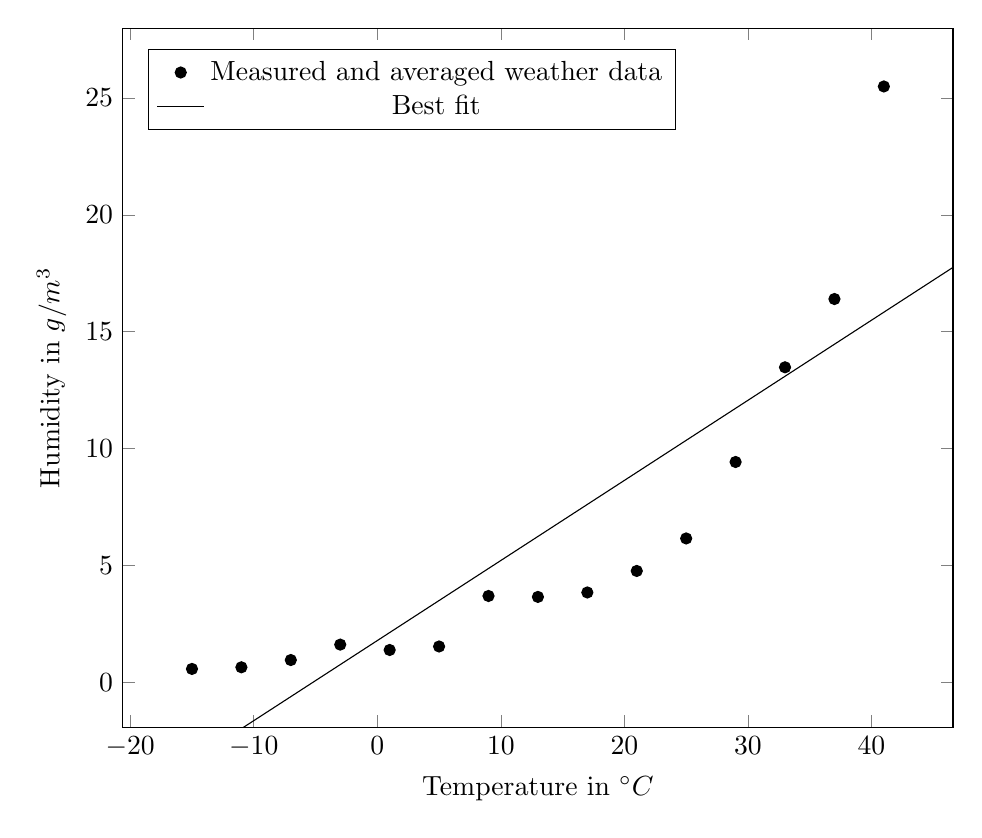
\begin{tikzpicture}
\begin{axis}
[ xlabel = Temperature in $ ^{\circ} C$,
ylabel = Humidity in $g/m^3$,
legend pos = north west,
xmin=-20.6, xmax=46.6,
ymin=-1.911, ymax=27.980999,
width=1\textwidth
]
\addplot[
only marks,
error bars/.cd,
 y dir=both,y explicit,
x dir=both,x explicit,
]
coordinates{
(-15,0.58) +- (0,0)
(-11,0.65) +- (0,0)
(-7,0.96) +- (0,0)
(-3,1.62) +- (0,0)
(1,1.39) +- (0,0)
(5,1.54) +- (0,0)
(9,3.7) +- (0,0)
(13,3.66) +- (0,0)
(17,3.85) +- (0,0)
(21,4.77) +- (0,0)
(25,6.16) +- (0,0)
(29,9.43) +- (0,0)
(33,13.48) +- (0,0)
(37,16.4) +- (0,0)
(41,25.49) +- (0,0)
};
\addlegendentry{Measured and averaged weather data}
\addplot[
domain=-20.6:46.6,
]
{x*0.34252678571428574 + 1.792485119047619}
;
\addlegendentry{Best fit}
\end{axis}
\end{tikzpicture}
\caption{Environment data of one year by a franconian weather station Thomas Karb 11.5.23}
\label{fig:EnvironmentRegression}
\end{figure}


\end{document}